\section{Механика}
След като дефинирахме основно приближение в нашия, можем да преминем към изграждането на математическия
модел и последващото му решаване. Такъв един модел се поддава добре на разглеждане от гледна точка на
диференциалната геометрия. Физичният смисъл на това е, че се фокусираме върху взаимодействието на материални
точки (,,частици``) в рамките на апроксимацията на непрекъснатите среди (следствията от това приближение
ще бъдат дискутирани по-нататък в текста). 
Освен това ще бъдат разгледани само дисперсионните взаимодействия (т.нар $r^{-6}$) взаимодействия).

\begin{figure}[h]
    \centering 
    \subfigure[Схема на взаимодействието]{\label{fig:cylinder_front}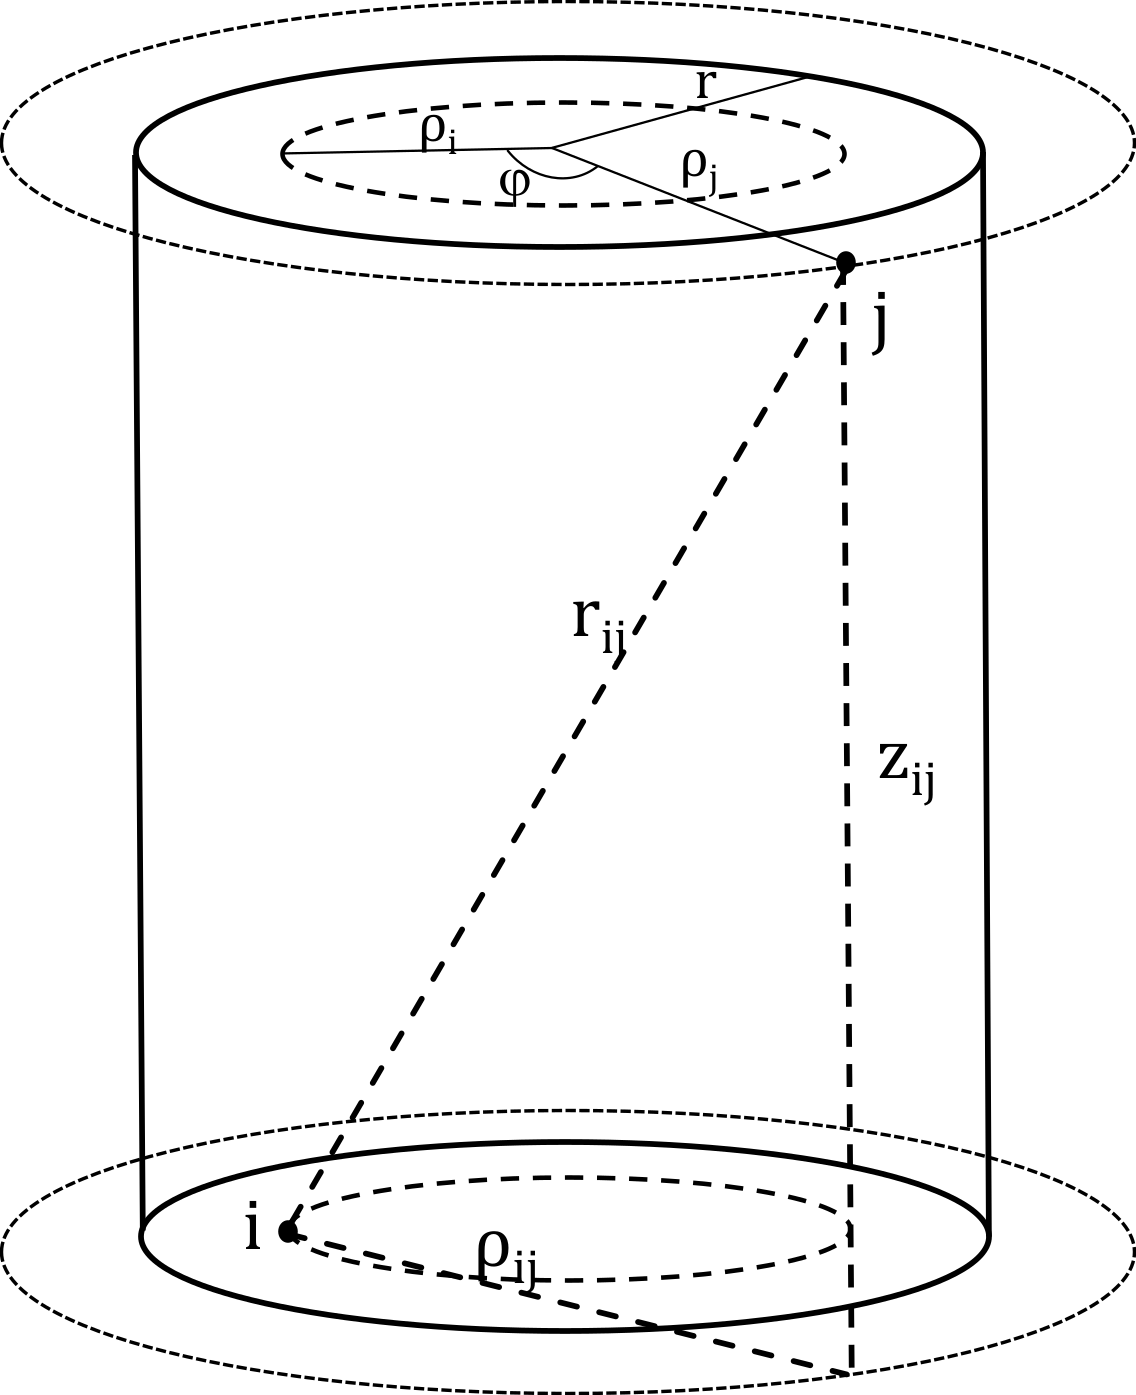
\includegraphics[width=0.48\linewidth]{cyl_fig_front.png}}
    \subfigure[Ортогонална проекция]{\label{fig:cylinder_top}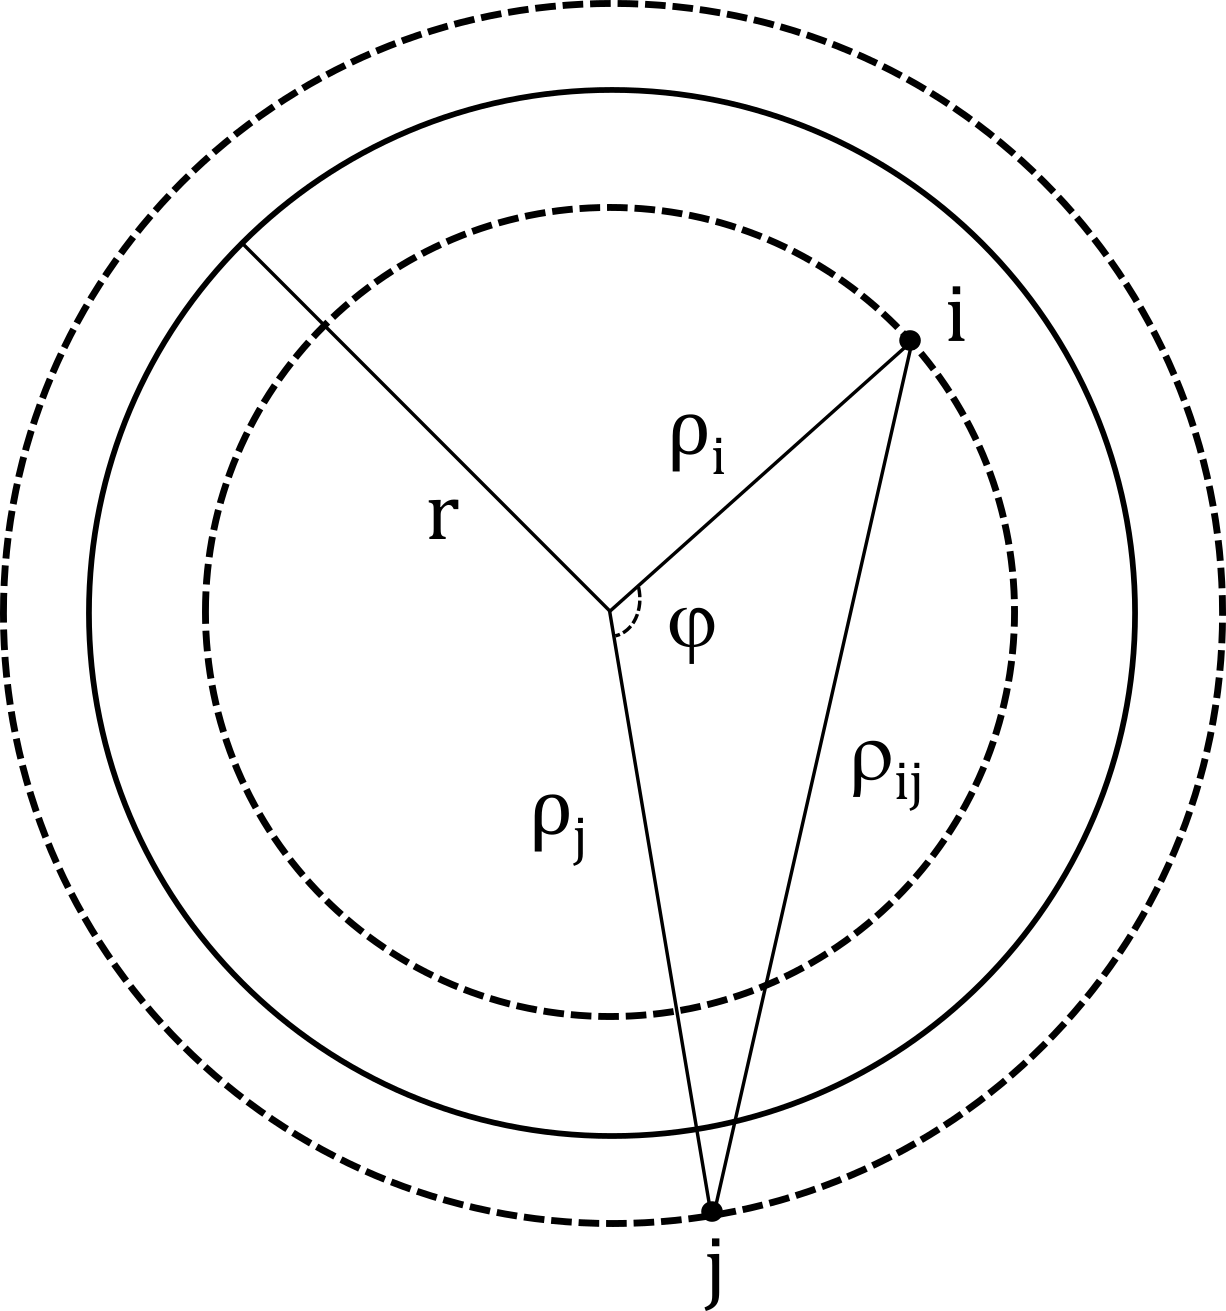
\includegraphics[width=0.48\linewidth]{cyl_fig_top.png}}
    \caption{
        Геометрична схема на разглежданата система. $r_{ij}$ - растояние между вътрешната \textbf{\textit{i}} и външната \textbf{\textit{j}} ,,частици``. $z_{ij}$ и $\rho_{ij}$ са съотвените проекции. $r_{ij}^2 = \rho_{ij}^2 + z_{ij}^2$. \textbf{\textit{r}} - радиус на цилиндъра.}
    \label{fig:cylinder_schematic}
\end{figure}

Такова разглеждания са правени много за случая на плоскопарелелните течни филми \cite{rusanov_shchekin}, като най-интересни са ,,тънките`` филми поради значителното влияние на капилярните
явления в тези системи. ,,Тънки`` (капилярни) са тези системи, чиито размери поне по едно от направленията са достатъчно малки, 
за да се наблюдава припокриване между двете междуфазови преходни области. В тях няма изотропен/обемен флуид, т.е. свойствата в тях са изцяло анизотропни. 
Всички ,,интересни`` капилярни явления всъщност са следствие от тази анизотропност на средата. 

Тук следва да отблежим, че механичния подход за тези системи е особено подходящ, тъй като в термодинамичния такъв губим детайлната информация за анизотропията - в случая на плоските филми
,,заместваме`` системата с опростена такава - обемен флуид ,,затворен`` между две математически равнини. От друга страна термодинамичния модел е удобен от практическа гледна точка - параметрите и енергиите
са 